%!TEX program = xelatex
\documentclass[10pt, compress]{beamer}

\usetheme{m}

\usepackage{booktabs}
\usepackage[scale=2]{ccicons}
\usepackage{minted}

\usemintedstyle{trac}

\title{Reconhecimento da Fala a Partir de Espectrograma usando MobileNetV2}
\subtitle{Projeto Demonstrativo 6 - Visão Computacional}
\date{\today}
\author{Igor Bispo  \and igor.rabbit99@gmail.com \\ Hevelyn Sthefany \and hevelyn.sthefany@gmail.com}

\institute{
  Departamento de Ciência da Comptutação\\
  Universidade de Brasília\\
  Campus Darcy Ribeiro, Asa Norte\\
  Brasília-DF, CEP 70910-900, Brazil,}

\begin{document}

\maketitle

\begin{frame}[fragile]
  \frametitle{Sumário}
  \tableofcontents
\end{frame}




\section{Reconhecimento da Fala} %-----------------------------------------------------------

\begin{frame}[fragile]
  \frametitle{Reconhecimento da Fala}
  \begin{center}O reconhecimento de fala é uma tecnologia que procura identificar palavras faladas em um áudio e convertê-las em texto.\end{center}

  \begin{figure}
  \centering
  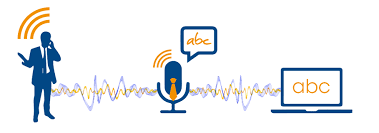
\includegraphics[scale=0.5]{images/speechrec.png}
    %\caption{Rotated square from
    %\href{http://www.texample.net/tikz/examples/rotated-polygons/}{texample.net}.}
  \end{figure}
\end{frame}


\begin{frame}
  \alert{Siri}, \alert{Open Mic+}, \alert{Siri}, \alert{Siri} são exemplos de aplicações que usam reconhecimento da fala.
\end{frame}


\begin{frame}{Reconhecimento com Espectrograma usando MobileNetV2}
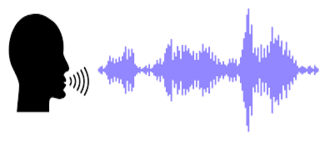
\includegraphics[scale=0.35]{images/process-11.png}
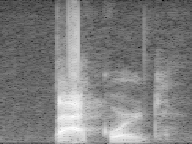
\includegraphics[scale=0.15]{images/process-2.png}
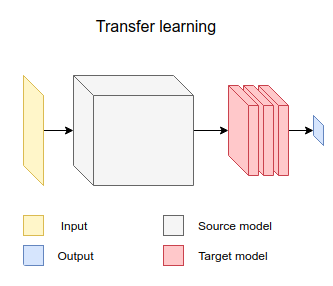
\includegraphics[scale=0.3]{images/process-3.png}

\includegraphics[scale=0.01]{images/process-4.jpg}
\end{frame}


\section{Espectrograma} %---------------------------------------------------------------------
\begin{frame}{Espectrograma}
\centering
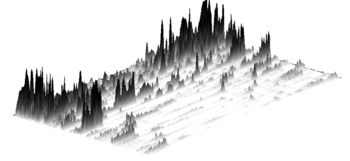
\includegraphics[scale=0.4]{images/spect1.png}
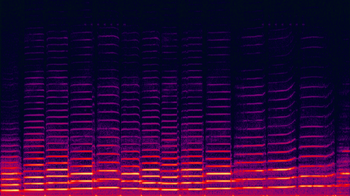
\includegraphics[scale=0.4]{images/spect2.png}
\\
\begin{center} Gráficos que analisam dinamicamente a densidade espectral de energia. Os valores são indicados no plano \alert{tempo} X \alert{frequência} e cores indicam \alert{intensidade} da densidade espectral de energia. \end{center}
\end{frame}

\begin{frame}
\centering
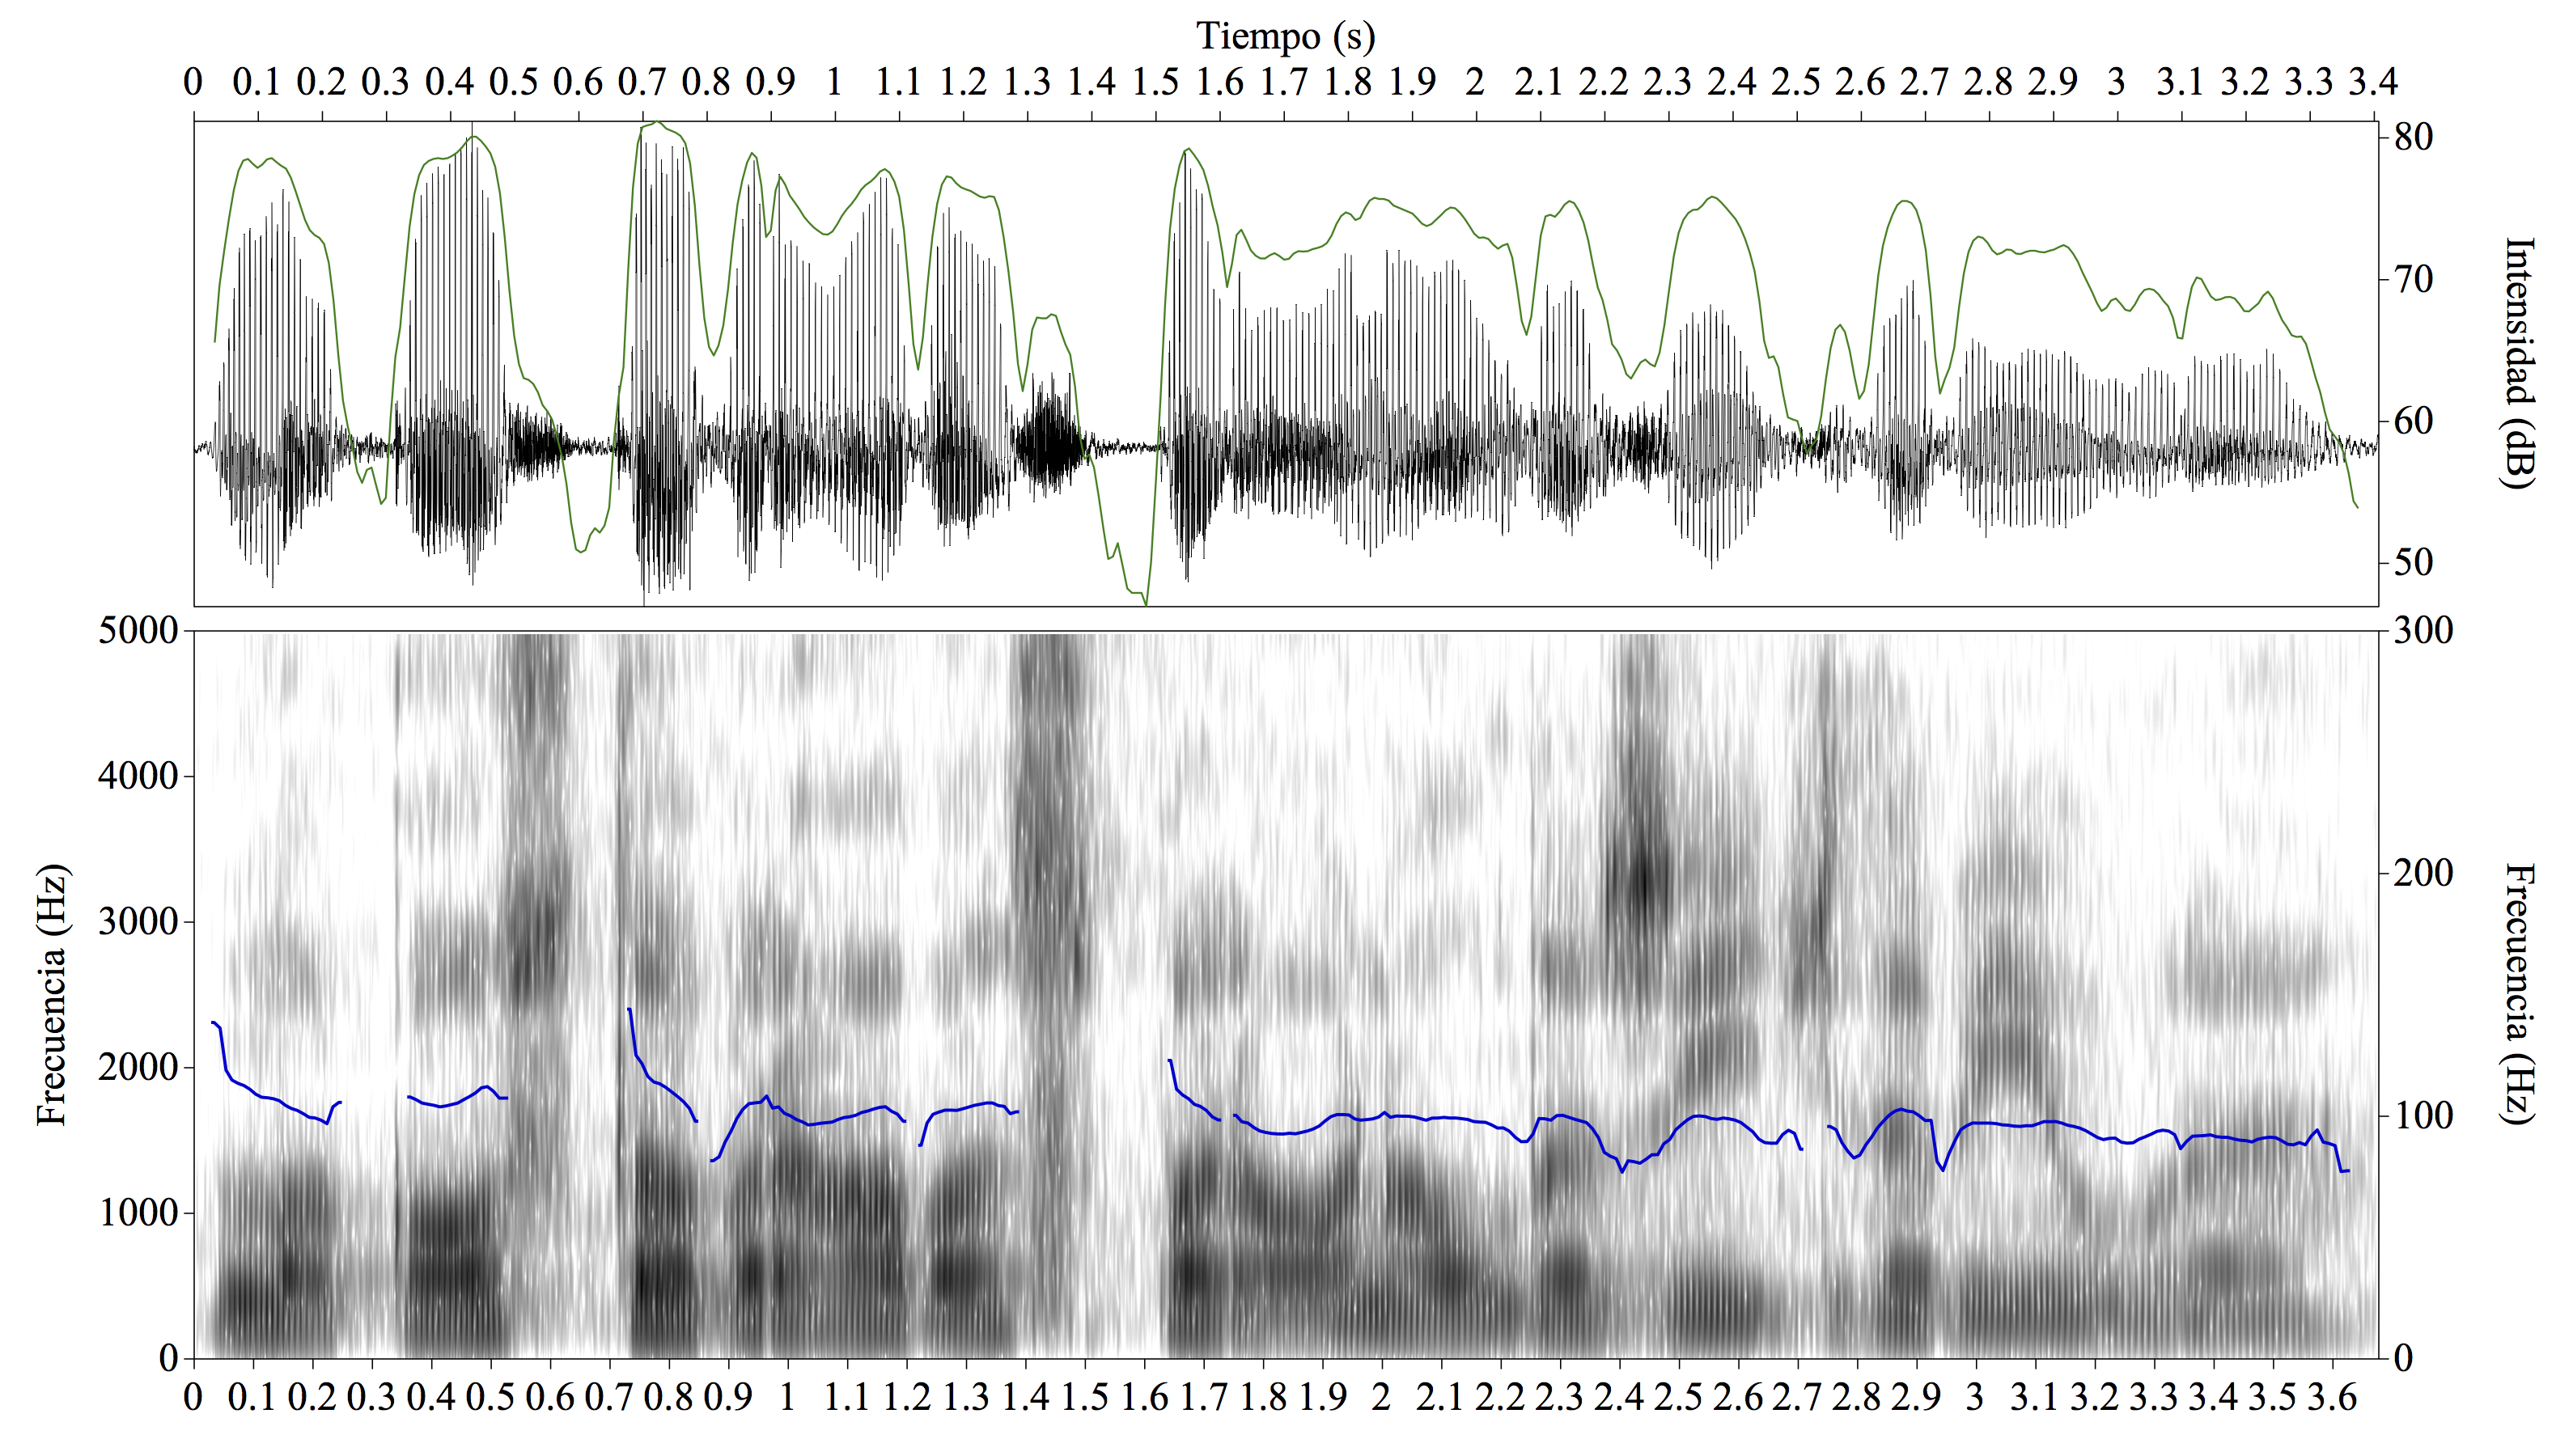
\includegraphics[scale=0.1]{images/spect3.jpg}
\end{frame}

\section{MobileNetV2} %---------------------------------------------------------------------
\begin{frame}{MobileNetV2}
  \begin{description}
    \centering
    \item[Convoluções Separáveis em Profundidade] São duas etapas:
          \begin{itemize}
          \item {\bf Convolução em profundidade} Mapeia uma única convolução em cada canal de entrada separadamente,
          \item {\bf Convolução Pontual} Convolução com um tamanho de kernel de 1x1 que combina os recursos criados pela convolução em profundidade.
          \end{itemize}
    \item[Resíduos Invertidos] Blocos residuais conectam o início e o fim de um bloco convolucional com uma conexão de salto.
    \item[Gargalos] Última convolução de um bloco residual tem uma saída linear antes de ser adicionada às ativações iniciais.
  \end{description}
\end{frame}





\begin{frame}{Convoluções Separáveis}


\end{frame}

\begin{frame}{Resíduos Invertidos e Gargalos}


\end{frame}

\section{Resultados}
\begin{frame}{Relatório de Classificação}


\end{frame}

\begin{frame}{Matriz de Confusão}


\end{frame}


%\plain{Dark background}{\vspace{-2em}\begin{center}\includegraphics[width=\textwidth]{images/valley.jpg}\end{center}}

\section{Conclusão}

\begin{frame}{Summary}

  Get the source of this theme and the demo presentation from

  \begin{center}\url{github.com/matze/mtheme}\end{center}

  The theme \emph{itself} is licensed under a
  \href{http://creativecommons.org/licenses/by-sa/4.0/}{Creative Commons
  Attribution-ShareAlike 4.0 International License}.

  \begin{center}\ccbysa\end{center}

\end{frame}


\plain{}{Obrigado!}

\end{document}
